% to choose your degree
% please un-comment just one of the following
\documentclass[bsc,frontabs,twoside,singlespacing,parskip,deptreport]{infthesis}     % for BSc, BEng etc.
% \documentclass[minf,frontabs,twoside,singlespacing,parskip,deptreport]{infthesis}  % for MInf

\usepackage{hyperref}
\usepackage{cite}
\usepackage{amsmath}
\usepackage{graphicx}
\usepackage{caption}
\usepackage{subcaption}
\usepackage{wrapfig}
\usepackage{tikz}
\usepackage{pgfplots}


\pgfplotsset{percentgraph/.style={%
        width=0.93\textwidth,
        ylabel={\% Messages Delivered},
        ymin=0,ymax=100}}

\begin{document}

\title{Targeted Influence in Social Networks}

\author{Lewis Barker}

% to choose your course
% please un-comment just one of the following
%\course{Artificial Intelligence and Computer Science}
%\course{Artificial Intelligence and Software Engineering}
%\course{Artificial Intelligence and Mathematics}
%\course{Artificial Intelligence and Psychology }   
%\course{Artificial Intelligence with Psychology }   
%\course{Linguistics and Artificial Intelligence}    
\course{Computer Science}
%\course{Software Engineering}
%\course{Computer Science and Electronics}    
%\course{Electronics and Software Engineering}    
%\course{Computer Science and Management Science}    
%\course{Computer Science and Mathematics}
%\course{Computer Science and Physics}  
%\course{Computer Science and Statistics}    

% to choose your report type
% please un-comment just one of the following
%\project{Undergraduate Dissertation} % CS&E, E&SE, AI&L
%\project{Undergraduate Thesis} % AI%Psy
\project{4th Year Project Report}

\date{\today}

\abstract{

}

\maketitle

\tableofcontents

%\pagenumbering{arabic}


\chapter{Introduction}
\section{Concept}
This project looks at the problem of directing messages across a social network via users' interactions, with the aim of reaching specific targets. This can be explained simply in terms of a real social network, such as Facebook. Initially some party has a message they wish to show to a specific person. However if the target does not know the originating party  then showing it directly to them, such as in an advert, will probably result in it being ignored. On the other hand, if one of the target's friends on Facebook shares the message and they see it, then they are more likely to notice it. However first, the message must reach one of the target's friends. To do this, the message must be shared by a number of intermediary users.


One of the main difficulties is that users do not see everything that their friends share - they will likely only look at some of the top items on their "news feed" before running out of attention. If there are a large number of messages shared by a user's friends, then since not all of them will be seen, not all of them can be passed on. To ensure that as many messages reach their target as possible, the amount of "noise" seen by a user must be reduced - in other words a message is only shown to them where it is beneficial to delivering that message. This is achievable by utilising the fact that in most social networks a user's "news feed", rather than being random, is generated by some complex algorithm. By modifying this algorithm and deciding what to show to each user, messages can be directed towards their destinations.

Since each message only needs to reach the destination once, the best way to reduce noise might be to find the shortest path from source to destination, and show it only to the next user along this path at each step. The problem with this is that even among those messages seen by a user, they may not share them all for one reason or another. Over enough steps a single copy of a message will likely get lost, and so it must be duplicated to increase the chance of delivery as much as possible. The algorithm now has to balance duplication of messages to avoid loss and avoiding unnecessary noise due to duplication.

\begin{figure}
\begin{tikzpicture}
\end{tikzpicture}
\begin{tikzpicture}
\end{tikzpicture}
\caption{TODO: Insert diagram. Should show multiple paths, some failing to share, and not showing message to unneeded nodes}
\label{fig:intro_example}
\end{figure}

This problem can be formalised using a graph to represent the social network, and having a number of messages at each node at any time in the process. The messages then move from one node to the next based on algorithms used to describe the actions of the user and the social network. Figure \ref{fig:intro_example} shows an example of this with a single message. Here red nodes have the message, blue nodes do not, and the yellow node is the target. The message moves through adjacent nodes until it reaches the target.

This project aims to specify this problem in more detail, develop an algorithm which can deliver as many messages as possible, and test and analyse this algorithm.

\section{Applications}
An effective algorithm which solves this problem has many applications. The most obvious way to use it is for targeted advertising. While this type of information spread in social networks is often used for general viral marketing, it may be the case that making a specific individual aware of some product is particularly advantageous. This method could then be used to direct it to them, without it seeming like they are being shown "adverts". This is particularly useful when considering individuals with large amounts of influence, such as a celebrity. Significant research has gone into identifying these influential users within social networks\cite{InfluenceMaximisation1, InfluenceMaximisation2, LabelledInfluenceMaximisation}. These studies generally consider how a message spreads from an initial person or set of people, and try to find the people who maximise the amount the message will spread. In other words, if a message can be delivered to an influential user, they can cause a cascade allowing it to reach many others. This results of this project could be used to direct the message to those influential people.

A different approach could be to use this method in a more charitable way, such as raising awareness of a some cause. Again this can be done in a viral way using information spread in networks, and influential users could again be targeted to spread the message further. In addition however, certain individuals may be known to be at more risk of some condition, and so spreading awareness to them would be particularly effective. Alternatively, certain users in a social graph will be positioned in such a way that they have a high probability of detecting a "contagion" spreading through it in early stages - identifying these users has been the subject of some research \cite{OutbreakDetection}. Spreading related information to these users may be an effective way to combat such contagions.

Finally, it may be possible to combine this method with graph summarisation techniques\cite{GraphSummary}. These involve condensing a large graph into a smaller one, in which super-nodes represent sets of nodes which had similar connections in the original graph. Using a summarised graph to represent the social network would still retain the connectedness properties that allow the method to work, but have other advantages. Communities would be targeted rather than individuals - for example rather than targeting a certain at-risk user with an awareness message, a group who are similarly at-risk might be targeted. This would also reduce the size of the problem, potentially making complex algorithms more feasible for large networks.

\section{Related Literature}
The concept of spreading information, or rumours, which is at the core of this project, has been investigated in many forms. An early example of this is \cite{Pittel87}, which looks at spreading a single rumour to all of a population of involved people.The paper uses a process consisting of discrete rounds, in which each individual who is informed of the rumour passes it on to another participant at random (who may or may not already be informed). The number of rounds required for there to be a high probability that the rumour spreads from a single person to all people involved are investigated, and a bound on this is proved. In \cite{KarpSSV00} a similar process is investigated, again looking at spreading a single rumour to all participants. A random phone call model is used, in which every round each player contacts another at random. In the \textit{push} scheme the caller passes the rumour on to the callee (as in \cite{Pittel87}), and in the \textit{pull} scheme rumours are only spread from callee to caller. A \textit{push\&pull} scheme combines these, allowing information to spread in either direction. A further more advanced scheme is also considered, which spreads the rumour in a more robust manner. Both of these papers looks at similar concepts to this project, however they differ in several ways. Both allow any player to contact any other, rather than having a social network of allowed communication; and both focus on spreading a single message to every player rather than many messages to specific targets.

There are also studies on spreading information in this way through social networks. An example is \cite{SocialNetworkRumours}, which considers the push and pull schemes as described above, but does so within a Preferential Attachment network, used to simulate a social network. This makes it more similar to the graph-based problem this project investigates, however again it only considers single messages spreading to all users.

An aspect of this project which is less common in literature is considering the limited attention of users in the network. The paper \cite{AllocatingAttention} looks at a form of this. Rather than using rounds, content is created and users consult their neighbours (using a pull scheme) according to Poisson processes. The attention limit is in the form of a limit to the sum of a user's rates of consulting their neighbours - however within this limit, attention may be allocated as desired. Cost for each user is defined in terms of how quickly any new content reaches them, and a social cost for the whole network in terms of how quickly content reaches all users. The paper investigates the cost when each user allocates their attention selfishly (to minimise their own cost) compared to the optimal cost, for several different graph types. This is similar to the system considered in this project - multiple messages interact at once, and users cannot see all of them at once due to limited attention. However the continuous process and lack of targets make the way the system is considered quite different.

Another less common aspect is targeting users within the social network. The paper \cite{TargetedSignedNetworks} looks at this idea of sending a message from source to target, but in the context of signed networks. Here each connection in the social graph is either "positive" or "negative" - signifying the type of relationship between the two individuals. If a message is passed to a user via someone they have a negative relationship with, then it will cause the recipient to lean towards the opposite view - and then that opposite view may be passed across another negative relationship, returning to the original. The paper looks at algorithms to create a path from the source to destination which minimises the distance while resulting in a positive influence on the target. While this contains the targeting aspect of this project's problem, the users in this paper are assumed to act in the optimal way which the algorithm wants them to - there is no random interactions. In this sense, while the algorithm may still be useful in some cases, it is a less realistic approach.

\section{Overview}
%In the remainder of this report, the work done up to this point in the project is presented, along with what work is to be done next. In Chapter 2 the formal definitions formulated for this project are covered in detail.
%
%Section 2.1 looks at the problem model itself, as it is used in later definitions and experiments. Section 2.2 describes the Kleinberg small world graph that was used to model the social network for this project. Secctions 2.3 and 2.4 then describe the user models used to define the sharing process, and the showing algorithms for deciding which messages to show each user - one of the main focuses of this project.
%
%Chapter 3 looks at the experiments carried out, first describing the simulation program used to carry these out in section 3.1, followed by presenting and discussing the results received in section 3.2.



\chapter{Formal Definitions}
\section{Problem Model}

\subsection{Problem Statement}
Initially we are given a \textbf{graph} $G = (V, E \subseteq V \times V)$ and $k$ \textbf{messages} $ m_{1} ... m_{k}$, which have \textbf{sources} $s_{1} ... s_{k}$ and \textbf{destinations} $d_{1} ... d_{k}$. 

The graph $G$ represents the social network, with vertices in $V$ being the users of the network and edges in $E$ being connections between users within the network. A connection between two users $a$ and $b$ means in our context that user $a$ may see some content shared by user $b$ - however whether they actually see it or not is decided by the social network's algorithm.

We wish to move these messages through the network so that as high a percentage as possible reach their final target.

\subsection{Rounds}
The system progresses in a series of \textbf{rounds}, representing periods of time passing in which messages can be passed on to other users. This allows us to more easily reason about the flow of information and also simulate the process.

For any round $t$, and for some vertex $v \in V$, the \textbf{shared set} $S_{t}(v)$ is the set of messages which were shared by $v$ in that round.

We assume that the source of a message will invariably share it initially (otherwise it has no chance to propagate). Therefore initially, at round 0, for each $v \in V$ the shared set is defined as the set of messages for which $v$ is the source:

\begin{equation}
S_{0}(v) = \{m_{x} \; | \; x \in [0, k] \wedge s_{x} = v\}
\end{equation}


We also define, for each $v \in V$ at any round $t > 0$, the \textbf{possible set} as all of the messages shared by neighbours of $v$ in the previous round - all the messages which $v$ may be able to see at this point:

\begin{equation}
P_{t}(v) = \bigcup_{u \in N(v)} \quad \bigcup_{m \in S_{t-1}(u)} (u, m)
\end{equation}

In the above equation, $N(v)$ is the set of neighbouring vertices of v, and $(u, m)$ is a 2-tuple. Given a tuple $p = (u, m)$, we say that $p_{(1)} = u$ and $p_{(2)} = m$, as a way of accessing the parts of the tuple.

Which of these messages are actually shown to $v$ is determined by the social network's algorithm - which is what we wish to design. We define the \textbf{shown set} of a user $v$ at some round $t$, $T_{t}(v)$, as the result of this algorithm - this will be a subset of the possible set for that user and round:

\begin{equation}
T_{t}(v) \subseteq P_{t}(v)
\end{equation}

Finally, from the messages that are shown to a user, the user will share some of them. This is decided by the user model algorithm. The result of this form the \textbf{shared set} of that user for this round - all messages in the user's shared set must have been part of their shown set for that round:

\begin{equation}
\forall m \in S_{t}(v) . \exists (u, n) \in T_{t}(v) . m = n
\end{equation}

This is then used as the basis for the possible set of neighbouring vertices in the next round. With this, we need only define the showing and user model algorithms to be able to simulate the spread of messages throughout the network.

\section{Network Graph} \label{sec:graph_def}
An important factor in how a message showing algorithm performs is the network that it is being performed on. If the network has invalid properties, the a successful algorithm may not be successful on other networks.

For the majority of this project, Kleinberg's model for small world graphs was used\cite{Kleinberg00}. This is a model which randomly creates a graph that fits certain properties. Initially, nodes are arranged in a grid layout, with a "grid distance" from each other. Each node is connected to its immediate neighbours (those a grid distance of 1 away). Each node is then connected to a constant number $k$ of other nodes. The probability of connecting node $u$ to node $v$ in this way is proportional to $d(u, v)^{-q}$ where $d(u, v)$ is the grid distance between $u$ and $v$, and $q$ is a constant affecting how likely the links are to be "far-reaching". If $q$ is 0, then the node will be linked to other nodes uniformly. If $q$ is high, the long links are more likely to connect closer nodes.

\begin{figure}[ht]
  \centering
    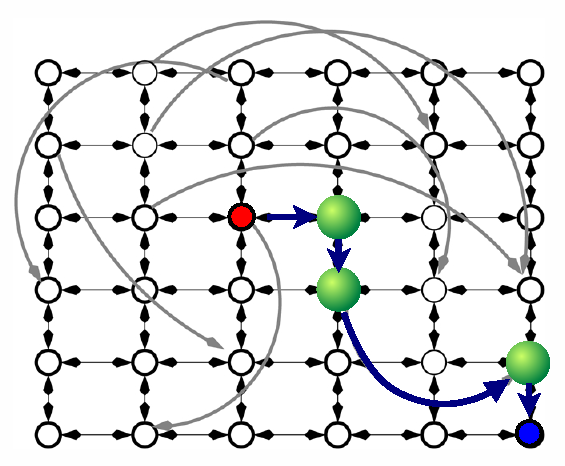
\includegraphics[width=0.5\textwidth]{Schabanel11_Kleinbergs_Network}
  \caption{A Kleinberg Graph with an example of the distributed greedy search\cite{Schabanel11}}
\end{figure}

This model provides several properties which make it suitable to use in place of a social network. Since it is randomly generated, we can run experiments using multiple different graphs to avoid results being skewed by peculiarities of individual networks. 

Additionally it fits into a category of graphs know as "Small World" graphs. This is related to Milgram's famous "Six Degrees of Separation" experiment\cite{Milgram67,TraversMilgram69}, in which he randomly chose individuals and asked them to forward a message on to a certain "target" via people they knew. Of those messages that reached the target, the median number of "steps" required was 6, displaying the existence of short paths within social networks - a fact that has also been seen in other studies\cite{MilgramBackup1,MilgramBackup2}. In addition to these paths existing, the experiment showed that it was possible for the intermediate individuals to find these paths without knowing the full structure of the network - they were able to conduct a distributed search. 

Kleinberg's model replicates both of these properties. For $q = 2$ and $k \ge 1$ the expected diameter of a graph generated using this model is $\theta (\log n)$ and a route between two nodes can be found in a distributed manner using $\theta (\log^{2}n)$ steps\cite{AnalyzingKleinberg}. This is achieved by sending the message as close as possible to the destination (in terms of grid distance) at each step.

This can be related to real networks intuitively. Individuals are more likely to be connected to those "close" to them - which in turn forms clusters of connections - but there will also be some "long-distance" connections that can connect clusters. To send a message to a far away target, a reasonable strategy would be to send to the person you know who is "closest" to the target - they are more likely to be connected to them.

While Kleinberg's small world model has been used primarily up to this point, other graph types may provide additional interesting insights. For example, using a plain grid could provide a baseline for what can be expected, to see if the algorithm developed takes advantage of the long link properties of the network. Alternatively, an real social network dataset could be used to see if the algorithm also work in actual networks.

\section{User Models} \label{sec:user_models}
While the main focus of this project was on the effect of the social network's "showing" algorithm, the model used also requires an algorithm to represent the user's actions. This algorithm should decide which of the messages shown to a user they then share - it chooses $S_{t}(v)$ based on $T_{t}(v)$. Depending on how this decision is modelled, it can add an element of uncertainty or randomness to the system, affecting which "showing" algorithms perform well.

\subsection{Basic User Model}
Initially, a very basic random selection method was used to choose the $S_{t}(v)$. Firstly, the user only considers the top $a$ of the messages shown to them (or all of the messages if there is less than $a$), where $a$ is a global constant - this represents the user's "attention", being unable to look at every message shown to them. In the implementations used, the value of $a$ is also known to the showing algorithm, which does not show more than this many messages. From these $a$ messages, $b$ are selected at random and shared (or all of them are shared if there are less than $b$), where $b$ is a global constant and $b \le a$.

This provides us with a degree of randomness - if there are more than $b$ messages shown to the user, we can't tell which ones will be passed on. However in the case where there are less than or equal to $b$ messages shown to the user, this model acts unrealistically - the user will share every message they see. A real social network user would likely be less predictable (unless there was some incentive to share messages), and may not share all of the messages in nay circumstances. As a result of this unnatural behaviour, showing each message to only a single user at each step was found to be a highly effective strategy - however in a real situation this would likely result in losing the message at an uncooperative user.

\subsection{Probabilistic User Model}
A more realistic user model can be created using more probabilistic methods. In this user model, the concept of a maximum attention of $a$ is retained, with the user considering up to $a$ messages. However from these $a$ messages, rather than choose a set amount at random each message is shared with a probability $p$, where $p$ is a global constant.

This results in a situation where a user may share all the messages they see, or may share none. This emulates how a user will only share certain messages based on some criteria unknown to the network. With this model, if messages are not sent to enough users then they are likely to not be shared and be lost.

\section{Showing Algorithms} \label{sec:showing_algorithms}
The key part of this project is the algorithm which decides which messages to show to each user. Users have "attention" limits, meaning that they will only look at a certain (globally constant) number of messages each round. This means that we can't just pass on every message - we need to prioritise. Each user is therefore only shown messages up to the "attention limit" to represent this. By changing which messages are shown we can attempt to direct messages to their recipients, preferably without clogging up the network with numerous duplicates and without losing the message by not duplicating it enough.

So far, several simple algorithms have been investigated, using basic heuristics to decide whether or not to show a message to a user.

\subsection{Algorithm 1: Any Closer Node}
In the first algorithm used, for each node we first select candidate messages that might be shown to them. A message is made a candidate if it has not already been delivered, and the receiving node (the one potentially being shown the message) is closer to the message's final target than the previous node was (the one that shared the message in the previous round, causing this message to be part of the possible set). After candidates have been selected, if there are more messages than can be shown to the node, the maximum amount are chosen randomly from the candidates. More formally:

\begin{equation}
\begin{split}
candidates = \{ (u, m_{k}) \in P_{t}(v) \:\: | \:\: & D(v, d_{k}) < D(u, d_{k}) \: \wedge \\
& m_{k} \mbox{ has not been delivered} \}
\end{split}
\end{equation}

\begin{equation}
T_{t}(v) = sample(candidates, max(||candidates||, a))
\end{equation}

Where $D(u, v)$ is the grid (Manhattan) distance between $u$ and $v$, $sample(x, n)$ randomly samples $n$ values from the collection $x$, and $a$ is the maximum messages that can be shown to any node (their attention span).

Note that if a message is in the possible set multiple times (from different previous nodes), it may be shown to the user multiple times (once for each previous node). Depending on the user model, this may increase the probability of it being shared by them.

\subsection{Algorithm 2: Further Nodes With Probability}
The second algorithm is a modification of the first with the intention of allowing the messages to spread in other directions not necessarily towards their destination. This may help prevent the message from dying out if the "direct" route is very busy.

In this algorithm, we again select candidates to be shown to each node. Again, messages are only made candidates if they have not been delivered. Of those undelivered messages, any for which the receiving node is closer to the destination than the previous node are made candidates, as before. Additionally, messages which will not get closer to their destination are made candidates with a globally constant probability $p$. As before, if there are too many candidates then the correct amount are chosen at random. More formally:

\begin{equation}
\begin{split}
candidates = \{ (u, m_{k}) \in P_{t}(v) \:\: | \:\: & (D(v, d_{k}) < D(u, d_{k}) \: \vee \: r < p) \: \wedge \\
& m_{k} \mbox{ has not been delivered} \}
\end{split}
\end{equation}

\begin{equation}
T_{t}(v) = sample(candidates, max(|candidates|, a))
\end{equation}

Where $0 \leq p < 1$ is a globally constant probability and $0 \leq r < 1$ is a randomly chosen value.

Note that if $p$ were to be set to 0, Algorithm 2 would behave the exact same as Algorithm 1.

\subsection{Algorithm 3: Only Single Best Node}
The third algorithm tested uses a simpler concept - each message is passed on to at most one other node, the node which is determined to be the "best" next step. This provides a basis for comparison with the case where messages are never duplicated.

Candidate messages are again selected for each node. In this algorithm a message is a candidate if it has not yet been delivered, and if that node is the "best" next step for the message. We define the "best" next step as the neighbour of the previous step which is closest to the target in grid distance, and in the case of a draw has the lowest node index (to ensure that the "best" next step is consistent). If there are too many candidates then the first up to the limit are taken. Since we are not worried about spreading messages "fairly" as they do not duplicate, this doesn't need to be chosen randomly. Formally:

\begin{equation}
\begin{split}
candidates = \{ (u, m_{k}) \in P_{t}(v) \:\: | \:\: & isBest(m_{k}, u) \: \wedge \\
& m_{k} \mbox{ has not been delivered} \}
\end{split}
\end{equation}

\begin{equation}
T_{t}(v) = candidates[:a]
\end{equation}

Where $isBest(m, u)$ is a predicate which is true if node $u$ is the best next step for message $m$, and $x[:a]$ is the first $a$ items in $x$.


\chapter{Implementation}
For the purpose of running simulations of message spread in networks, a program was written allowing for running various simulations and receiving relevant results. The program was written in Python, using the NetworkX library\cite{NetworkX} to represent and manipulate the network graphs. The program is split into classes, many of which have abstract base classes, to allow for easily creating different versions to swap in and out.

There is a \texttt{GraphGenerator} abstract base class, subclasses of which encapsulate the knowledge specific to the graph model being used - including how to create a graph of that type, and how the nodes should be positioned in the visualisation (for example if the network is based on a grid layout, it should be positioned as such). The rest of the program is totally independent from this knowledge, meaning that by simply using a different subclass the graph generation method can be modified completed - for example the graph could be loaded from a static file.

The showing algorithms are contained within subclasses of the \texttt{ShowModel} class, the main method of which is \texttt{show\_alg} which given a user's possible set and some additional information about the state of the network, returns a subset of the messages to be shown to them. Similarly, the user models algorithms are represented by subclasses of the \texttt{ShareModel} class, which has a method \texttt{share\_alg} to take the shown set and return the messages which the user will share. Changing which of these subclasses is used in the simulation allows comparing the performance of different algorithms.

These classes are brought together by the \texttt{Simulation} class, which is given an instance of each of \texttt{GraphGenerator}, \texttt{ShowModel}, and \texttt{ShareModel} on creation. The simulation can then be either run once or repeated multiple times, collating the results. When repeating the simulation, it can set to either use the exact same network graph or to regenerate the graph using the same generation method - in the case of randomly generated graphs, this allows for repeating the simulation to remove random differences caused by specific graphs. The simulation class can also create visualisations as outputs. It can output either images of the state at each round of the simulation, or a single video of the entire simulation. In these visualisations, a single message is highlighted as it spreads through the network, while the other vertices are coloured based on their level of traffic. This allows for seeing how a message moves through the graph and how far it spreads, as well as where potential bottlenecks occur and how busy the network is as a whole.


\chapter{Results}
After development of the algorithms, experiments were run to compare their performance. Experiments were also run to ensure that the parameters chosen were reasonable and would give valid results. Unless otherwise stated all simulations were run until any action had completely stopped - that is, no messages were seen in some round by any node, either due them being delivered already or dying out before delivery. Also, unless otherwise stated, all simulations were run 20 times and the average result taken, to avoid random fluctuations.

For a large number of experiments, Kleinberg's graph model, as described in Section \ref{sec:graph_def}, was used. In all of these experiments, $k=1$ and $q=2$ were used, where $k$ is the number of "long links" created from each node and $q$ "clustering exponent", which is used alongside the grid distance between two nodes to calculate the probability of there being a long link between them. As is shown in \cite{Kleinberg00},  $q=2$ is the the "sweet spot" for a graph based on a 2 dimensional lattice, at which decentralised routing can achieve delivery times polynomial in $\log n$. Additionally $k$ must be set to a small constant, so $k=1$ was chosen. A 20 by 20 grid was used to create the graph from, as this size was found to be large enough to provide good results, but not so large that the experiments took an excessively long time to run.


\section{User Model Comparison}
The two models of message sharing by users, as described in Section \ref{sec:user_models}, were compared to each other experimentally to decide which was a better fit for future experiments. This was conducted by running separate simulations using showing algorithms 1, 2, and 3 as described in Section \ref{sec:showing_algorithms}. The purpose of these experiments was to document how the success of each user model changes as messages are spread more or less. It was hypothesised that since the basic user model shares all messages when there are very few shown to it, then limiting the spreading of messages to one copy per distinct message would give good results. However this would not match the expected result on real humans - somewhere along the chain a user would be expected to not share a message, due to not liking the contents or something similar.

First, the basic user model was tested. This model uses two variables: $a$, the maximum messages that each user will "see" or consider as candidates to share; and $b$, the maximum number of messages that the user will share (where $b \leq a$). If less than or equal to $b$ messages are shown then all will be shared, otherwise from the first $a$ messages, $b$ are randomly chosen to be shared. For these experiments the values $a = 20$ and $b = 5$ were used - they were chosen arbitrarily, as the purpose of these results is not to compare the different user models or parameters directly, but to see how the results for each model change as the amount of message spread changes. It was tested against four different showing algorithm setups: Algorithm 1, which potentially shows only messages to users closer to their destination (equivalent to Algorithm 2 with $p=0$); Algorithm 2 with $p=0.4$, where $p$ is the probability of a message being a candidate to be shown to a user not closer to the destination; Algorithm 2 with $p=0.6$; and Algorithm 3 where each message is shown to exactly one other user each round. To determine whether nodes are "closer" or not, the grid position based distance measure was used in all cases. These simulations all used distinct Kleinberg's model graphs.

\begin{figure}
\begin{subfigure}[]{0.45\textwidth}
\begin{tikzpicture}
\begin{axis}[percentgraph,xmin=0,xmax=800,xlabel={Message Count}]
\addplot table [x=Message count, y=average delivered (percent), col sep=comma] {results/user_model/BasicShare_Prob0.csv};
\end{axis}
\end{tikzpicture}
\caption{Algorithm 1}
\end{subfigure}
%
\begin{subfigure}[]{0.47\textwidth}
\begin{tikzpicture}
\begin{axis}[percentgraph,xmin=0,xmax=800,xlabel={Message Count}]
\addplot table [x=Message count, y=average delivered (percent), col sep=comma] {results/user_model/BasicShare_Prob40.csv};
\end{axis}
\end{tikzpicture}
\caption{Algorithm 2 -- $p=0.4$}
\end{subfigure}
\par\bigskip 
\begin{subfigure}[]{0.47\textwidth}
\begin{tikzpicture}
\begin{axis}[percentgraph,xmin=0,xmax=800,xlabel={Message Count}]
\addplot table [x=Message count, y=average delivered (percent), col sep=comma] {results/user_model/BasicShare_Prob60.csv};
\end{axis}
\end{tikzpicture}
\caption{Algorithm 2 -- $p=0.6$}
\end{subfigure}
%
\begin{subfigure}[]{0.47\textwidth}
\begin{tikzpicture}
\begin{axis}[percentgraph,xmin=0,xmax=800,xlabel={Message Count}]
\addplot table [x=Message count, y=average delivered (percent), col sep=comma] {results/user_model/BasicShare_OnlyBest.csv};
\end{axis}
\end{tikzpicture}
\caption{Algorithm 3}
\label{subfig:basic_user_model_3}
\end{subfigure}
\caption{Results using the basic user model}
\label{fig:basic_user_model}
\end{figure}

The results for the basic user model can be seen in Figure \ref{fig:basic_user_model}. Each graph shows the percentage of messages delivered as the initial message count is increased from 25 to 800, in steps of 25. The 4 subfigures show the performance of the different showing algorithms. From this we can see that as the probability of spreading messages away from the target increases (from 0, to 0.4, to 0.6), the number of messages delivered in general decreases. However if only one copy of each message is shown each round, as shown in  Subfigure \ref{subfig:basic_user_model_3}, the percentage of message delivered increases drastically.

Next the probabilistic user model was tested. Again, $a=20$ was used for the maximum number of messages "seen" by each user. For the probability of sharing each message seen, $p=0.5$ was used. The same showing algorithms, distance measure, and graph setup were used as for the basic user model.

\begin{figure}
\begin{subfigure}[]{0.45\textwidth}
\begin{tikzpicture}
\begin{axis}[percentgraph,xmin=0,xmax=800,xlabel={Message Count}]
\addplot table [x=Message count, y=average delivered (percent), col sep=comma] {results/user_model/ProbShare_Prob0.csv};
\end{axis}
\end{tikzpicture}
\caption{Algorithm 1}
\end{subfigure}
%
\begin{subfigure}[]{0.47\textwidth}
\begin{tikzpicture}
\begin{axis}[percentgraph,xmin=0,xmax=800,xlabel={Message Count}]
\addplot table [x=Message count, y=average delivered (percent), col sep=comma] {results/user_model/ProbShare_Prob40.csv};
\end{axis}
\end{tikzpicture}
\caption{Algorithm 2 -- $p=0.4$}
\end{subfigure}
\par\bigskip 
\begin{subfigure}[]{0.47\textwidth}
\begin{tikzpicture}
\begin{axis}[percentgraph,xmin=0,xmax=800,xlabel={Message Count}]
\addplot table [x=Message count, y=average delivered (percent), col sep=comma] {results/user_model/ProbShare_Prob60.csv};
\end{axis}
\end{tikzpicture}
\caption{Algorithm 2 -- $p=0.6$}
\end{subfigure}
%
\begin{subfigure}[]{0.47\textwidth}
\begin{tikzpicture}
\begin{axis}[percentgraph,xmin=0,xmax=800,xlabel={Message Count}]
\addplot table [x=Message count, y=average delivered (percent), col sep=comma] {results/user_model/ProbShare_OnlyBest.csv};
\end{axis}
\end{tikzpicture}
\caption{Algorithm 3}
\label{subfig:prob_user_model_3}
\end{subfigure}
\caption{Results using the probabilistic user model}
\label{fig:prob_user_model}
\end{figure}

Figure \ref{fig:prob_user_model} shows the results for the probabilistic user model, again showing percentage delivered as message count increases for the 4 different showing algorithm configurations. This case shows an entirely different trend from the basic model - as the messages are spread away from the destination more, the number delivered increases. Also, the change in message count has less of an effect on the percent delivered than before. This suggest that in the basic model the main cause of failed delivery is being unable to show messages due to the users being at the attention limit - and so spreading messages more makes the situation worse. However in the probabilistic model, the main problem is messages not being passed on after the user sees them - and so spreading the messages further improves this.

Of particular note is the performance of showing algorithm 3 when the probabilistic user model is used, as seen in \ref{subfig:prob_user_model_3}. In this case the amount delivered is very low, as you would expect if each message was shown to only one person. This suggest that when the number of messages in the system is low, the probabilistic model is more realistic. Based on these results, the probabilistic user model is used for the remaining experiments.

\section{Showing Algorithm Comparisons}


\section{Distance Measure Comparisons}


% use the following and \cite{} as above if you use BibTeX
% otherwise generate bibtem entries
\bibliographystyle{plain}
\bibliography{reportBib}


\end{document}
